\let\negmedspace\undefined
\let\negthickspace\undefined
\documentclass[journal]{IEEEtran}
\usepackage[a5paper, margin=10mm, onecolumn]{geometry}
%\usepackage{lmodern} % Ensure lmodern is loaded for pdflatex
\usepackage{tfrupee} % Include tfrupee package

\setlength{\headheight}{1cm} % Set the height of the header box
\setlength{\headsep}{0mm}     % Set the distance between the header box and the top of the text

\usepackage{gvv-book}
\usepackage{gvv}
\usepackage{cite}
\usepackage{amsmath,amssymb,amsfonts,amsthm}
\usepackage{algorithmic}
\usepackage{graphicx}
\usepackage{textcomp}
\usepackage{xcolor}
\usepackage{txfonts}
\usepackage{listings}
\usepackage{enumitem}
\usepackage{mathtools}
\usepackage{gensymb}
\usepackage{comment}
\usepackage[breaklinks=true]{hyperref}
\usepackage{tkz-euclide} 
\usepackage{listings}                                  
\def\inputGnumericTable{}                                 
\usepackage[latin1]{inputenc}                                
\usepackage{color}                                            
\usepackage{array}                                            
\usepackage{longtable}                                       
\usepackage{calc}                                             
\usepackage{multirow}                                         
\usepackage{hhline}                                           
\usepackage{ifthen}                                           
\usepackage{lscape}
\usepackage{circuitikz}
\tikzstyle{block} = [rectangle, draw, fill=blue!20, 
    text width=4em, text centered, rounded corners, minimum height=3em]
\tikzstyle{sum} = [draw, fill=blue!10, circle, minimum size=1cm, node distance=1.5cm]
\tikzstyle{input} = [coordinate]
\tikzstyle{output} = [coordinate]
\renewcommand{\thefigure}{\theenumi}
\renewcommand{\thetable}{\theenumi}
\setlength{\intextsep}{10pt} % Space between text and floats
\numberwithin{equation}{enumi}
\numberwithin{figure}{enumi}
\renewcommand{\thetable}{\theenumi}

\begin{document}

\bibliographystyle{IEEEtran}
\vspace{3cm}

\title{1.5.18}
\author{EE25BTECH11030 - Josyula G S Avaneesh}
\maketitle

\subsection*{\textbf{Question:} } 
Find the coordinates of a point $A$ where $AB$ is the diameter of the circle whose center is  $\myvec{2\\-3 }$ and $B$ is the point $\myvec{1\\4}.$\\
\solution \\ 

\underline{\textbf{Theory :}} Center of a circle is the mid-point of the diameter. \\

Let $P$ be the center of the given circle , with $AB$ as the diameter.

Let $\vec{A}$ be the coordinates required to be found. 
\subsubsection*{Given }
 $B \equiv \myvec{1 \\ 4} , P \equiv \myvec{2\\-3}$ 
 
\text{If } $\vec{P}$ \text{is the mid point of } $\vec{AB}$ 

\begin{align}
    \vec{P} = \frac{\vec{A} + \vec{B}}{2}  
\end{align}

\begin{align}
    \vec{A}=2\vec{P}-\vec{B}
\end{align}

Substituting the given vectors , we get : 

\begin{align}
    \vec{A} = 2\myvec{2\\-3} - \myvec{1 \\ 4} \\ 
    \vec{A} = \myvec{ 4 - 1\\ -6 - 4  }      
\end{align}

\begin{align*}
        \therefore A \equiv \myvec{3\\-10}
\end{align*}

\textbf{Hence} , Coordinates of $A$ are $\myvec{3\\-10}$ 

\begin{figure}[H]
    \centering
    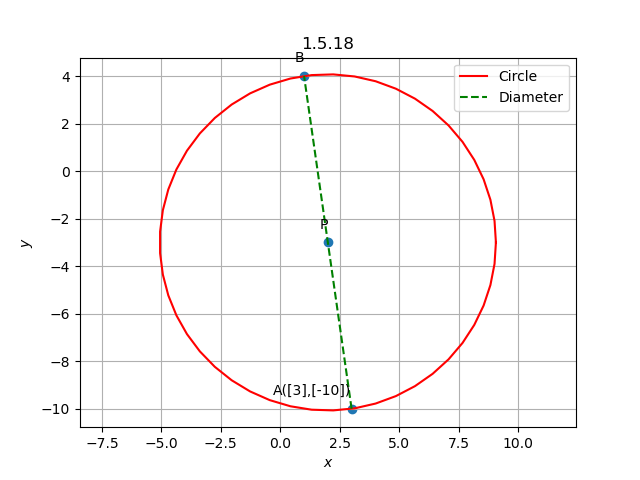
\includegraphics[width=1\linewidth]{figs/circle_graph2.png}
    \caption{Circle With Centre P}
    \label{fig:placeholder_1}
\end{figure}

\end{document}